\chapter{Imagefilm}
\section{Film, eine Einleitung}
\begin{quote}
    Ein Bild sagt mehr als tausend Worte
\end{quote}
\begin{flushright}
    Fred R. Barnard
\end{flushright}
Mit diesem Zitat lässt sich die Wichtigkeit des Films als kommunikationsmittel sehr gut beschreiben. So liefert ein Film nicht nur eine große Menge an Informationen durch Darstellung eines Bildes, sondern kann ein Film auch zeitliche Abläufe vermitteln. Oft haben Filme auch noch das weitere Medium des Tons, welches in sich nochmals mehr Informationen trägt. Ein Film kann deswegen als ein sehr \enquote{dichtes} Informationsträger angesehen werden, da in kurzer Zeit sehr viele Informationen gleichzeitig, teils durch verschiedene Kanäle wie Bild und Ton, übertragen werden. So ergibt auch der Einsatz dieses Mediums für die \ac{MOBTS} Konferenz in Mannheim Sinn.\\

Im Folgendem wird deshalb kurz die Geschichte des Films erläutert, um die Vorteile und die interessante Herkunft dieses Mediums darzustellen. Anschließend wird auf verschiedene Techniken des Filmens eingegangen, welche die Grundlagen der Filmproduktion darstellen. Danach wird auf die Umsetzung des Werbefilms für die \ac{MOBTS} Konferenz eingegangen, welcher anschließend bewertet wird. Zuletzt wird noch in einem Fazit ein kurzer Ausblick gegeben.
\section{Geschichte des Films}
Der Mensch suchte schon seit Ewigkeiten danach, seine Erfahrungen und Erlebnisse visuell darzustellen. So finden sich schon in den frühesten Zivilisationen verschiedenste Darstellungen der Umwelt. Noch bevor der Mensch Schrift erfand malte er auf Höhlenwände Bilder. Mit dem technischen Fortschritt entwickelte sich auch die Darstellungsformen, sodass Bilder auf Leinwände gemalt wurden, bis schließlich die Fotografie erfunden wurde. Bei der Fotografie wird ein lichtempfindlicher Film durch eine Linse mit Licht bestrahlt, was ein Abbild der Umwelt darstellt.\\
Um das Bild bewegt erscheinen zu lassen, erzeugt ein Film eine Illusion, indem mehrere aufeinanderfolgende Bilder schnell hintereinander dargestellt werden. Dies erscheint dann aber einer Bildrate von 24 Bildern pro Sekunde dem menschlichen Auge als flüssige Bewegung.\autocite{Schmidt.2013}\\
Auf der Suche nach dem allerersten \enquote{Film} gibt es drei wesentliche Kandidaten.\autocite{HeadsUp.} Der chronologisch erste Film wurde 1878 erstellt.\autocite{Muybridge.1878} Das Ziel dieses Films war es, herauszufinden, ob ein Pferd im Gallopp jemals mit allen vier Hufen gleichzeitig den Boden verlässt. Dafür Fotografierte Edward Muybridge ein Pferd in Palo Alto, Kalifornien im Lauf mehrfach mit verschiedenen Kameras, die entlang der Strecke aufgestellt waren. Diese verschiedenen Fotos wurden dann im Nachhinein schnell hintereinander gezeigt, um zu entdecken, dass ein Pferd mit allen vier Hufen gleichzeitig vom Boden abhebt. Hier war es jedoch nicht die Absicht von Muybridge, ein Bewegtbild zu erzeugen, weshalb dies oft nicht als erster Film angesehen wird.\\
Oft wird der Film Roundhay Garden Scene als der erste Film betitelt.\autocite{LePrince.1888} Der von Louis Amie Augustin Le Prince erstellte Film von 1888 geht zwar lediglich zwei Sekunden, stellt jedoch schon eine zusammenhängende Handlung dar und gilt deswegen als Film.\\
Etwas länger dagegen ist der Film \enquote{Arrival of a Train at A la Ciotat}, im original \enquote{L'Arrivée d'un Train A la Ciotat}, welcher 1895 von den Gebrüdern Lumiere erstellt wurde.\autocite{Lumiere.1895} Dieser 50-sekündige Film zeigt einen einfahrenden Zug, eine bekannte Alltagsszene. Zu diesem Film gibt es die unbestätigte Geschichte, welche besagt, dass die Zuschauer dieses Films von der Illusion in einem solchen Sinne getäuscht wurden, sodass sich Panik breit machte und einige Zuschauer aus Angst aus dem Theater flohen. Auch wenn diese Geschichte vielleicht nicht wahr ist, zeigt sie die Überzeugungskraft des Mediums und die Emotionen, die durch visuelle Einflüsse ausgelöst werden können.\\
Dieses Ziel blieb ein wichtiges Ziel in der Filmkunst und Regisseure versuchen bis heute, wirksam Emotionen in Zuschauern auszulösen.\\
\section{Techniken des Filmens}
\subsection{Framing}
Eine der elementarsten Techniken des Filmes ist die des Framings. Das Framing ist ein großer Teil des Filmemachens und beschäftigt sich damit, wie die Kamera eine Szene darstellt. Dabei geht es sowohl um den die Entfernung, Höhe, Brennweite, Fokuseinstellung, Position sowie um den Winkel der Kamera. Auch spielt hierbei oft das Blocking, also die Position der Schauspieler oder Objekte zueinander eine Rolle.\\
Bei der Aufnahmeweite, auch Shotsize genannt, unterscheidet man zunächst zwischen Landschaftsaufnahmen und Aufnahmen von Personen. Landschaftsaufnahmen wird in der Regel der Name Wide Shot oder Long Shot zugeordnet. Dabei wird noch weiter zwischen einem Extreme Wide Shot oder Extreme Long Shot und einem Long Shot unterschieden.

\begin{figure}[h]
    \centering
    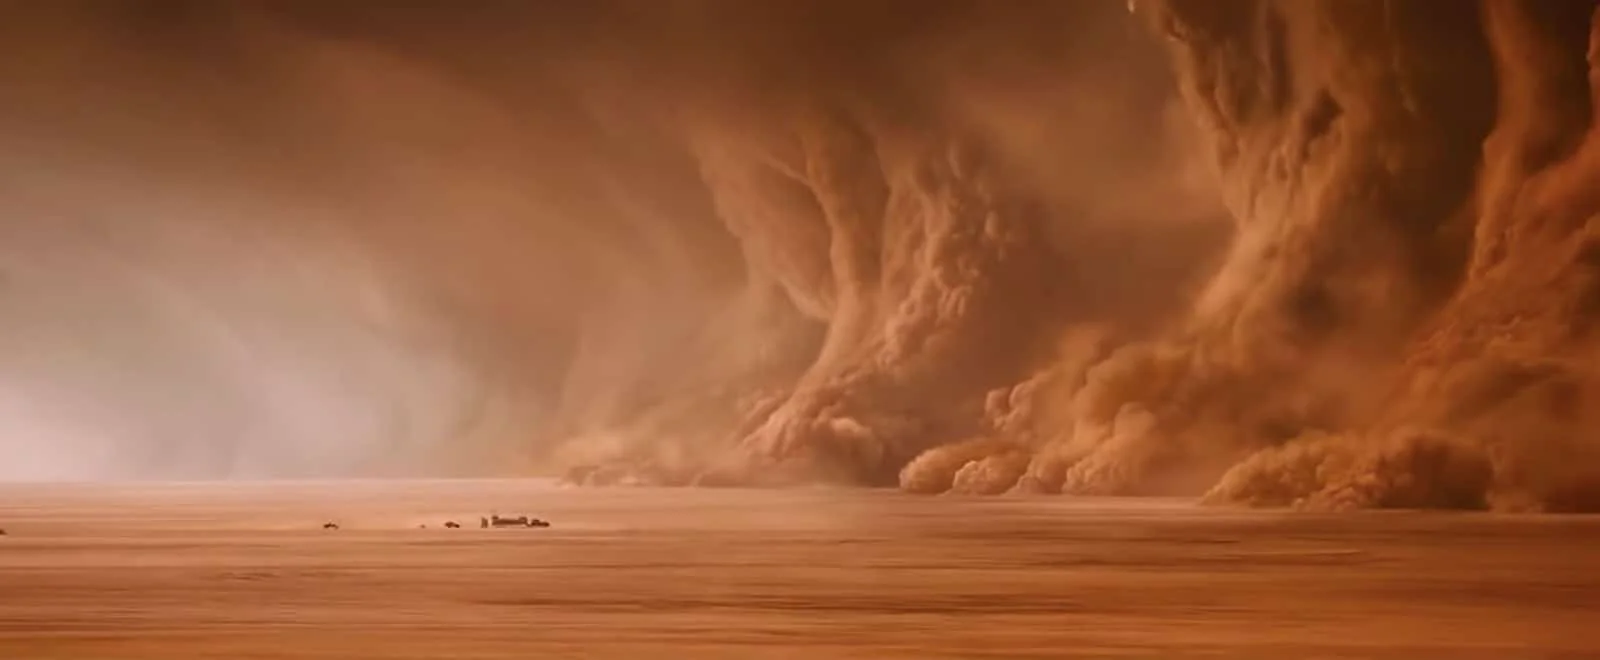
\includegraphics[width=0.8\textwidth]{img/AO_ELS.jpg}
    \caption[Imagefilm: Extreme Wide Shot]{Beispiel eines Extreme Wide Shot (EWS) aus dem Film \textbf{Mad Max: Fury Road}}
    \label{fig:AO_EWS}
\end{figure}

Wie in \autoref{fig:AO_EWS} zu sehen ist, wird in einem Extreme Wide Shot ein großer Teil der Landschaft gezeigt, während kleinere Objekte wie Schauspieler kaum erkennbar sind.\autocite{Studiobinder.2020}

\begin{figure}[h]
    \centering
    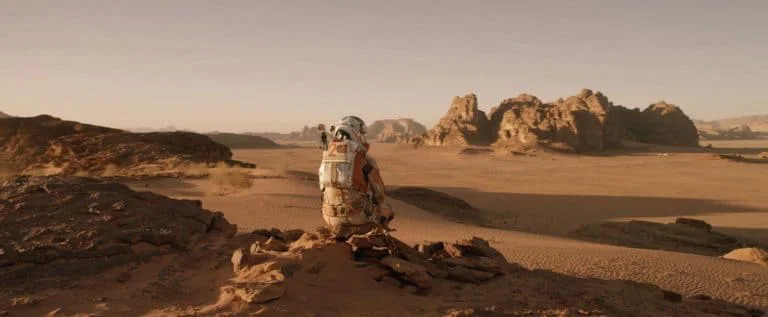
\includegraphics[width=0.8\textwidth]{img/AO_WS.jpg}
    \caption[Imagefilm: Wide Shot]{Beispiel eines Wide Shot (WS) aus dem Film \textbf{Der Marsianer}}
    \label{fig:AO_WS}
\end{figure}

Beim Wide Shot hingegen, wie in \autoref{fig:AO_WS} zu sehen ist, ist der Schauspieler noch gut zu sehen, während der Hintergrund, die Landschaft immer noch betont ist.\\
Diese beiden Aufnahmearten sind die beliebtesten Shots für Landschaftsaufnahmen und können in Verbindung mit anderen Shotarten kombiniert werden, um eine größere Variation von Shots zu erhalten.\\

Bei Personenaufnahmen wird zwischen mehr Shots unterschieden. 

\begin{figure}[h]
    \centering
    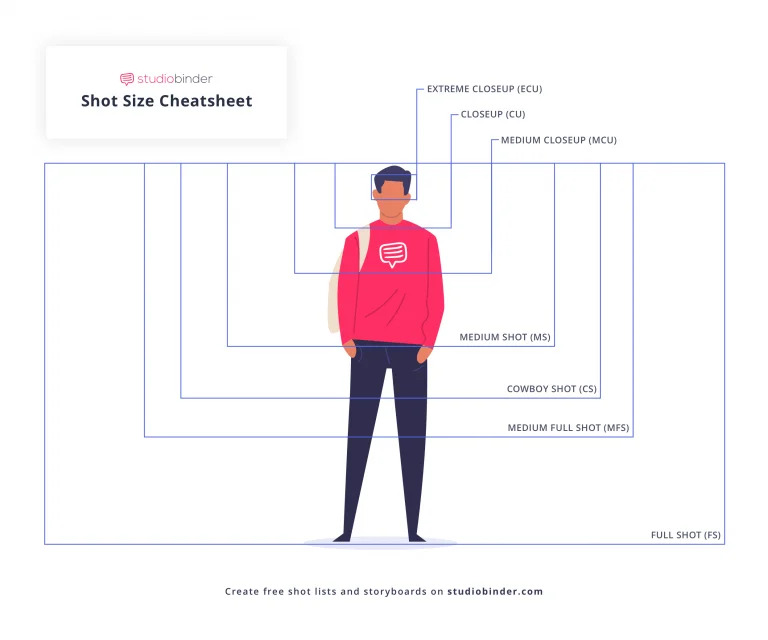
\includegraphics[width=1\textwidth]{img/AO_ShotOverview.jpg}
    \caption[Imagefilm: Shots Übersicht]{Übersicht der bekanntesten Shots für Personen}
    \label{fig:AO_WS}
\end{figure}

Dabei wird in 7 Hauptshots unterschieden, es können aber auch beliebige Zwischenstufen ausgewählt werden, welche dann in der Regel dem naheliegensten Shot zugeordnet wird. 

Der Full Shot ist der weiteste Shot, er zeigt am meisten. In dieser Aufnahme ist der ganze Charakter zu sehen, meistens wird dabei oben und unten noch ein wenig frei gelassen, um es nicht zu eng wirken zu lassen. 

Der nächste Shot ist der Medium Full Shot, hier wird der Charakter von den Knien bis zum Kopf gefilmt. Dieser wird oft benutzt, um Bewegungen eines Charakter zu zeigen.

Beim Cowboy Shot ist der Charakter von etwas unter der Hüfte bis zum Kopf zu sehen. Wie der Name schon sagt, wurde dieser Shot häufig in Western eingesetzt, um sowohl den Charakter als auch den Revolver eines Charakters zu zeigen. Ein Beispiel dafür kann in \autoref{fig:AO_CS} gesehen werden.

\begin{figure}[h]
    \centering
    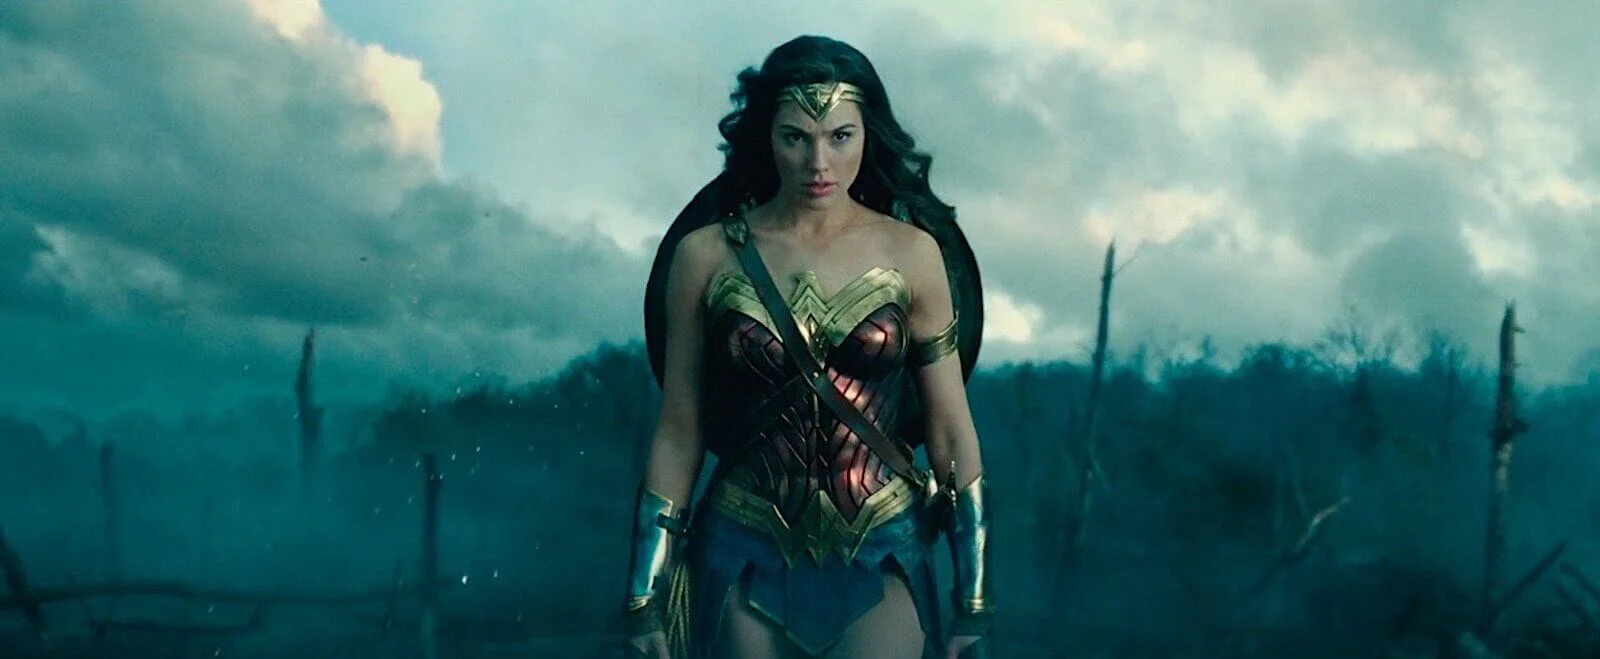
\includegraphics[width=0.8\textwidth]{img/AO_CS.jpg}
    \caption[Imagefilm: Cowboy Shot]{Beispiel für den Cowboy Shot aus dem Film \textbf{Wonder Woman}}
    \label{fig:AO_CS}
\end{figure}

Der Medium Shot wird öfter eingesetzt und zeigt den Charakter von der Hüfte bis zum Kopf. Dieser eignet sich für viele verschiedene Arten von Szenen, da sowohl das Gesicht wie auch der Oberkörper zu sehen ist.

Der Medium Close Up Shot zeigt den Charakter von den Ellenbogen bis zum Kopf und eignet sich somit hervorragend für Konversationen. Das Gesicht und der Oberkörper sind erkennbar, jedoch ist das Bild nicht zu nah, dass es ungemütlich wirkt. Es ist etwa die gleiche Ansicht, die ein Mensch haben würde, wenn er in einer normalen Konversation mit einem anderen Menschen ist. 

Der Close Up dagegen ist wesentlich näher und zeigt meistens nur das Gesicht des Charakters. Er kann auch genutzt werden, um die Detailansicht eines Gegenstandes oder anderen Körperteils zu zeigen. Er wird genutzt, um besondere Aufmerksamkeit auf dieses Objekt zu legen. Bei einem Close Up eines Charakters sollen oft die Emotionen des Charakters betont werden, da bei diesem Shot Gesichtsausdrücke sehr gut erkennbar sind. Das ist in \autoref{fig:AO_CU} zu sehen.

\begin{figure}[h]
    \centering
    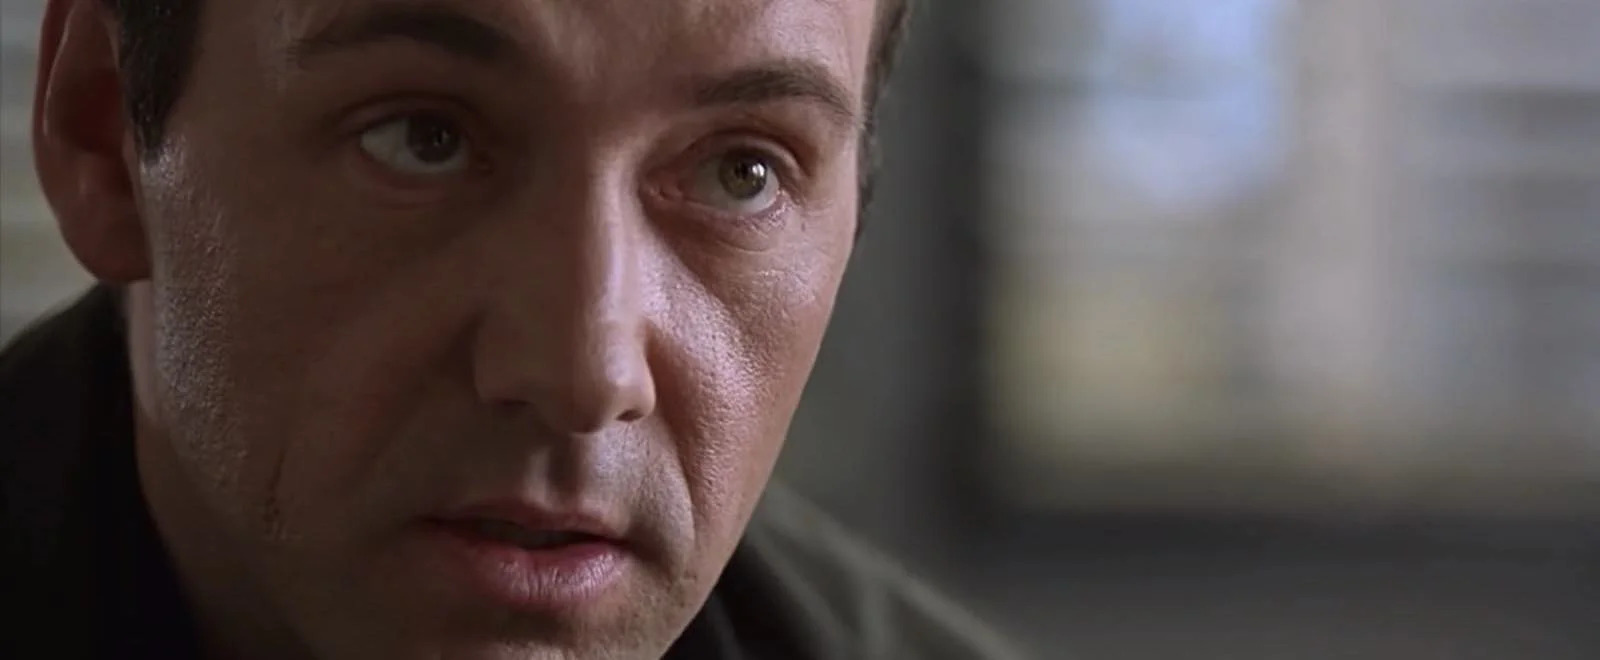
\includegraphics[width=0.8\textwidth]{img/AO_CU.jpg}
    \caption[Imagefilm: Close Up Shot]{Beispiel für den Close-Up Shot aus dem Film \textbf{Die Üblichen Verdächtigen}}
    \label{fig:AO_CU}
\end{figure}

Der Extreme Close Up Shot verstärkt dabei nochmal die Wirkung des Close Up Shots und lenkt somit noch mehr Aufmerksamkeit auf einen bestimmten Aspekt. Oft werden dabei die Augen dargestellt, um eine besonders starke Emotion herauszustellen.

Diese verschiedenen Shotsizes können für unterschiedliche Funktionen innerhalb eines Films genutzt werden.\autocite{Studiobinder.2020}

Eine wichtige Funktion ist dabei der Establishing Shot. Oft wird dieser als eigener Shot dargestellt, es handelt sich jedoch in der Regel um einen Wide Shot oder Extreme Wide Shot. Mit dem Establishing Shot soll eine Szene im Film etabliert werden. Mit diesem Shot soll der Zuschauer orientiert werden und der Schauplatz gezeigt werden. Oft ist es der erste Shot einer Szene oder eines Films.

Weitere wichtige Funktionen sind der Reaction Shot, also eine Aufnahme, die als direkte Reaktion auf die Handlung fungiert, auch Cut-Away genannt, sowie der Over-the-shoulder und Point-of-view shot, welche die Standpunkte der Charaktere besser vermitteln.
\subsection{Goldener Schnitt}
Der Goldene Schnitt ist ein Werkzeug, um ästethisch ansprechende Bilder zu gestalten.\autocite{Bruchwitz.2017}
Der Goldene Schnitt ist dabei eine mathematische Formel. Er beschreibt das Verhältnis von zwei Längen $a$ und $b$ zueinander. Dabei ist $b$ im Verhältnis zu $a$ genau so lang, wie $a$ zu $a + b$ ist. Daraus ergibt sich die Formel
\begin{equation}
    \frac{a}{b} = \frac{a+b}{a}
\end{equation}
Stellt man dieses Verhältnis in die zweite Dimension, so bekommt man ein zwei Rechtecke welche im Verhältnis des Goldenen Schnittes zueinander stehen. Wenn in dem jeweils kleineren Rechteckt auch wieder der Goldenen Schnitt gebildet wird und die Eckpunkte dieser geometrischen Form miteinander verbunden werden, so erhält man die sogenannte Spirale des Nautilus.

\begin{figure}[h]
    \centering
    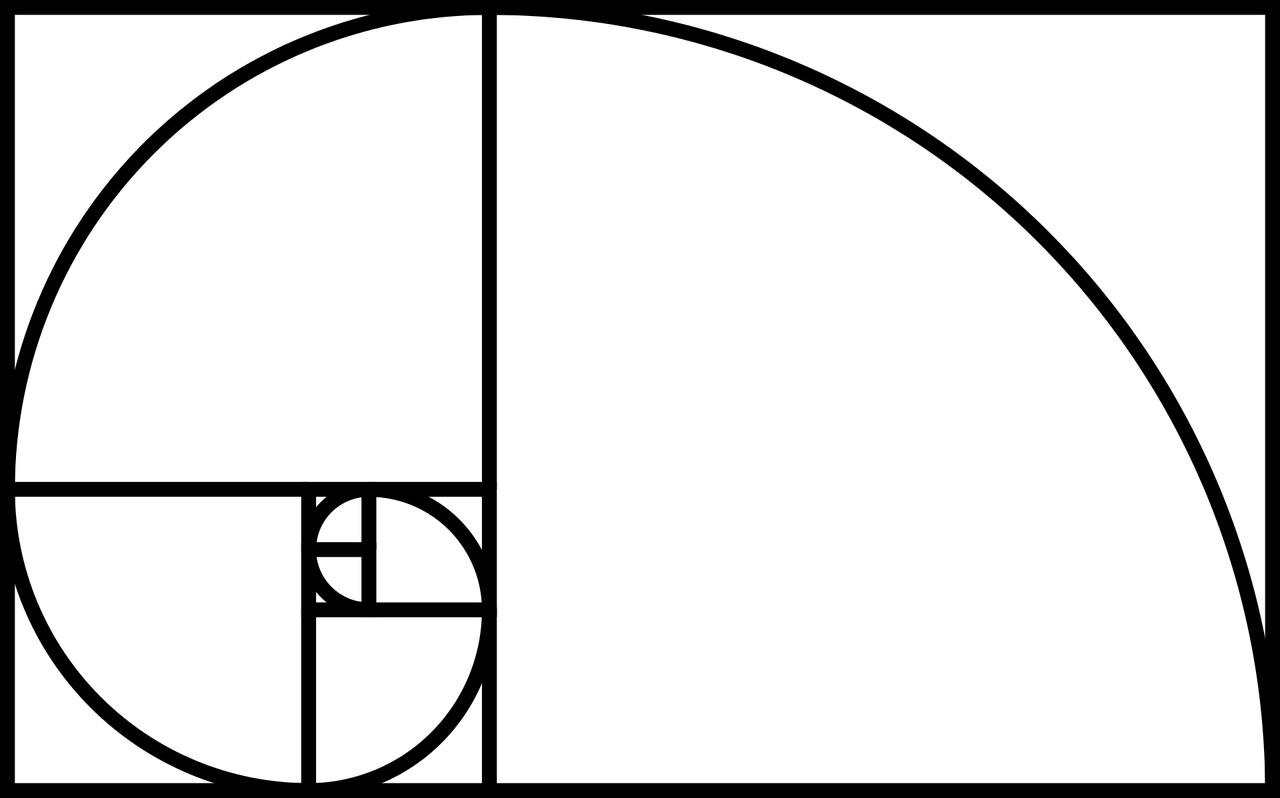
\includegraphics[width=0.6\textwidth]{img/AO_GoldenerSchnitt.jpg}
    \caption[Imagefilm: Der Goldene Schnitt]{Die Nautilus Spirale: eine zweidimensionale Darstellung des Goldenen Schnitts}
    \label{fig:AO_CU}
\end{figure}

\subsection{Skript und Storyboard}
\subsection{Schnitte und Übergänge}
\subsection{Voiceover}
\section{Imagefilm zur MOBTS}
\subsection{Ziel des Films}
\subsection{Skript des Films}
\subsection{Storyboard des Films}
\subsection{Durchführung und Produktion}
\section{Bewertung und Reflektion}
\section{Fazit und Ausblick}